\chapter{\kadaia}
\section{\purpose}
本章では,画像のカラーチャネル操作,量子化,階調反転,閾値処理を行う.またグレイスケール画像に対してヒストグラムを作成する.
\paragraph{\kadaiaa}RGB色空間の画像を,緑チャネルだけを抜き出してグレイスケール画像を作成する.赤チャネル,青チャネルについても同様にグレイスケール画像を生成する.さらに,RGB画像の赤チャネルと青チャネルを入れ替えたカラー画像を作成する.
\paragraph{\kadaiab}グレイスケール画像を生成する.緑チャネルは色の濃淡を多く含む.RGB色空間から色の濃淡を抽出したい場合は,緑(G)の成分を多く抽出するとよい.具体的な割合を,\eqref{equ:grayscale}に示す.ここではNTSC輝度信号を取り出す方法で行う.生成したグレイスケール画像に対して,画像の量子化数を変更することによる,画像の変化を確認する.量子化数は8Bit,4Bit,2Bit,1Bitの4種をテストする.量子化数1Bitの画像を2値画像という.
\begin{align}
    \textrm{Gray scale image} & = \textrm{Red}\times 30\% +\textrm{Green}\times 59\% +\textrm{Blue}\times 11\%\label{equ:grayscale}
\end{align}
\paragraph{\kadaiac}各量子化数の画像に対して,その画像を階調反転させる.階調反転とは,白黒を反転させることである.量子化数による階調変換後の画像を比較する.
\paragraph{\kadaiad}閾値処理とは,とある値(閾値)以上の場合を白,閾値以下を黒とし,2値画像を作成することである.
\paragraph{\kadaiae}量子化数8Bitのグレイスケール画像のヒストグラムを作成する.画素値\(n(n=0,1,\dots ,255)\)の画素が何画素含まれているかのヒストグラムを作成する.
\paragraph{\kadaiaf}自分が写っている写真と,背景だけが写っている写真の差分画像をとる.これを背景差分と呼ぶ.背景差分の後,閾値処理を行う.物体領域を正しく検出するために考慮する点を考察する.
\section{\method}
\paragraph{実験に用いる装置}このレポート内すべての実験にはMathWorks\raisebox{2mm}{\tiny\textregistered}社の\matlab を用いて,\tblref{tbl:実験環境}の環境下で実験する.
\begin{table}[H]
    \caption{実験環境}
    \label{tbl:実験環境}
    \begin{tabularx}{\textwidth}{AR}
        \hline
        実験機                      & MacBook Air 2022 (Apple社)\texttt{MLY13J/A}    \\
        プロセッサ                    & Apple Silicon M2\ \  8コアCPU,8コアGPU            \\
        メモリ                      & 8GB                                           \\
        \multirow{2}{*}{\matlab} & R2023a - academic use (Update1 9.14.02239454) \\
                                 & 64-bit (maci64) March 30, 2023                \\
        \hline
    \end{tabularx}
\end{table}
また,このレポートないすべての実験では\matlab でプロットしたグラフを出力するための\texttt{exportgraphics}関数,画像を書き出すための\texttt{imwrite}関数を用いる(\srcref{src:グラフ・画像出力}).
\begin{lstlisting}[numbers={none},caption={グラフ・画像出力},label={src:グラフ・画像出力}]
exportgraphics(figurename,'path/figure_name.pdf','ContentType','vector');
imwrite(data,"path/figure_name.png");
\end{lstlisting}
\paragraph{\kadaiaa}
\texttt{imwrite}関数を用いて,画像の読み込む.読み込んだ画像はRGB色空間で保存されており,チャネル1にはR,チャネル2にはG,チャネル3にはBが保存されている.
グレイスケール画像を作成するには,\eqref{equ:grayscale}の割合で画像を加算合成する.\mat{m}{n}の行列\texttt{A}に対して,\mat{1}{n}を取り出したければ,\verb|A(1,:)|と記述する.\verb|:|は,すべての要素を表す記号である.
赤チャネルと青チャネルを入れ替えるためには,赤チャネルの行列と青チャネルの行列を変数に保存し,それぞれ互いのチャネルに代入する.\scall{\kadaiaa}\sref{src:05_01}.

\begin{wrapfigure}{r}[0mm]{.3\textwidth}
    \centering
    \vspace{-.7cm}
    \begin{lstlisting}[caption={\texttt{bitshift}関数},label={src:bitshift}]
img = bitshift(img, n);
    \end{lstlisting}
    \vspace{-.5cm}
\end{wrapfigure}
\paragraph{\kadaiab}
量子化数を変更するために,\texttt{bitshift}関数を用いる(\srcref{src:bitshift}).
この関数は,\texttt{img}を左に\texttt{n}ビットシフトする関数である.右シフトしたい場合は\texttt{n}を負の数で与える.
ビットシフトについて,1ビット右シフトするごとにそのデータは\(1/2\)される.
これを利用して,量子化数4Bitの場合は右に4Bitシフト,量子化数2Bitの場合は右に6Bitシフト,量子化数1Bitの場合は右に7Bitシフトする.

\begin{wrapfigure}{r}[0mm]{.225\textwidth}
    \centering
    \vspace{-.5cm}
    \begin{tikzpicture}
        \coordinate (A) at (4,1);
        \draw (0,0.5)--(4,0.5);
        \draw (0,0)rectangle(A);
        \foreach \x in {1,2,...,8}
            {
                \draw (\x/2,0.4)--(\x/2,0.6);
                \draw (\x/2,1)--(\x/2,0.9);
                \draw (\x/2,0)--(\x/2,0.1);
                \node at ($(\x/2-1/2,0.5)!0.5!(\x/2,1)$){\texttt{1}};
                \node at ($(\x/2-1/2,0)!0.5!(\x/2,0.5)$){\ifnum\x<5\texttt{0}\else\ifnum\x>5\texttt{1}\else\ifnum\x=5\texttt{1}\fi\fi\fi};
            }
    \end{tikzpicture}
    \caption{4ビットシフト}
    \label{fig:4ビットシフト}
    \vspace{-.5cm}
\end{wrapfigure}
量子化数4Bitを例にあげる.仮に画素値が\texttt{255}(白)を持つ画素の場合,量子化数を4Bitにする,つまり4Bit右シフトすると,画素値は\texttt{15}になる(\figref{fig:4ビットシフト}).このままでは画素値の範囲が\(0\)から\(15\)となる.
この対策として,全体画素値と\(255/15\)の積を取ることで,画素値を\(0\)から\(255\)にスケーリングする.\scall{\kadaiab}\sref{src:05_02}.
\paragraph{\kadaiac}
各量子化数ごとに階調反転する.階調反転を実現するためには,階調反転した画像を\texttt{double}型に変換したあと,\(-1\)との積をとり,\(255\)を足した後で\texttt{unit8}型に変換する\footnote{その画像の各画素値が\texttt{double}型であるとき,\texttt{imwrite}が,データを自動的にリスケールし書き出すため.}.\scall{\kadaiac}\sref{src:05_03}.

\begin{wrapfigure}{r}[0mm]{.3\textwidth}
    \centering
    \vspace{-.7cm}
    \begin{lstlisting}[caption={判定結果の格納},label={src:判定結果の格納}]
mat = [1 2 3; 4 5 6; 7 8 9];
bin = mat > 5;
% -- 結果 --
bin = [0 0 0; 0 0 1; 1 1 1];     
    \end{lstlisting}
    \vspace{-.5cm}
\end{wrapfigure}
\paragraph{\kadaiad}
\matlab には,判定結果のブール値を行列に格納する機能がある.
\srcref{src:判定結果の格納}より,行列\texttt{mat}の各元が\(5\)より大きい箇所を\(1\),\(5\)以下のところを\(0\)とする行列\texttt{bin}を作成できる.この行列を真理行列と呼ぶ.
この機能を用いて,ある閾値に対して,閾値よりも大きければ\(1\)を戻し,閾値以下であれば\(0\)を戻す行列を作成する.画素値の範囲を\(0\)から\(255\)へするために,行列の各元と\(255\)の積をとる.今回は,閾値を\(64\),\(128\),\(192\)で実験する.\scall{\kadaiad}\sref{src:05_04}

\begin{wrapfigure}{r}[0mm]{.3\textwidth}
    \centering
    \vspace{-.9cm}
    \begin{lstlisting}[caption={\texttt{sum}関数},label={src:sum関数}]
matA = [1 2 3];
s_matA = sum(matA); 
% -> 出力:6
matB = [1 2; 1 1; 1 1];
s_matB = sum(matB); 
% -> 出力:[3 4]
s_s_matB = sum(sum(matB)); 
% -> 出力:12
    \end{lstlisting}
    \vspace{-.7cm}
\end{wrapfigure}
\paragraph{\kadaiae}
ヒストグラムを作成するために,この関数は行列の元を足し合わせる\texttt{sum}関数を用いる(\srcref{src:sum関数}).
各画素値\(0\)から\(255\)に対して,その画素値と等しい箇所を\(1\)とする真理行列を作成し,各元の和を\texttt{sum}関数を用いて算出する.
その結果が,ある画素値がいくつ画像に含まれているかを指す.
\paragraph{\kadaiaf}
固定カメラ\footnote{手での固定は,背景がズレる可能性があるので,カメラを固定して撮影した.}で撮影した写真を用いる.「背景と被写体が写っている画像\texttt{img\_sbj}」「背景のみの画像\texttt{img\_bg}」の2点を撮影した.背景差分画像は,\(\texttt{img\_sbj}-\texttt{img\_bg}\)で生成する.
生成した画像に対して,閾値処理する.閾値処理する前後での画像比較,閾値による比較し,考察する.今回,閾値を\(32\),\(64\),\(128\)で実験する.\scall{\kadaiaf}\sref{src:05_06}.
\section{\result}
\begin{figure}[h]
    \newcommand{\vsp}{\vspace{2em}}
    \centering
    \begin{minipage}[b]{.19\textwidth}
        \centering
        
\includegraphics[keepaspectratio,width=\textwidth]{../../kut.jpg}
        \subcaption{元画像}
        \label{fig:元画像}
    \end{minipage}
    \begin{minipage}[b]{.19\textwidth}
        \centering
        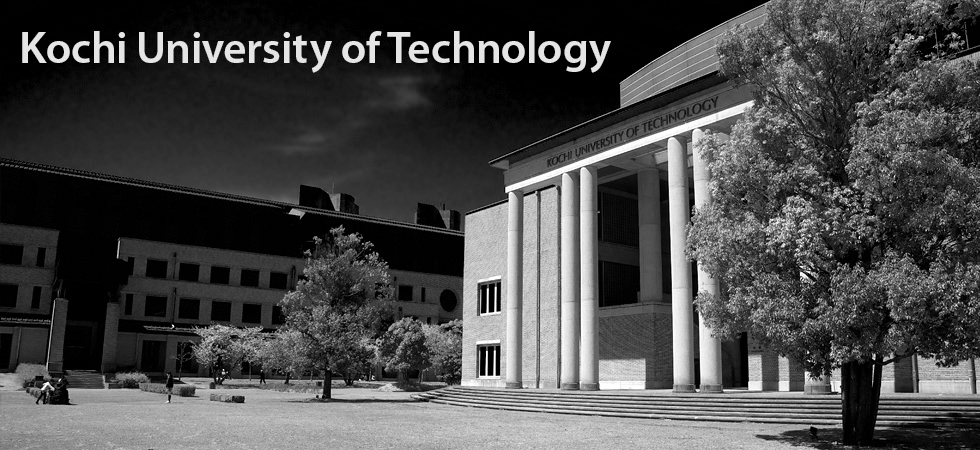
\includegraphics[keepaspectratio,width=\textwidth]{../../Figures/05_11_r.png}
        \subcaption{赤チャネル}
    \end{minipage}
    \begin{minipage}[b]{.19\textwidth}
        \centering
        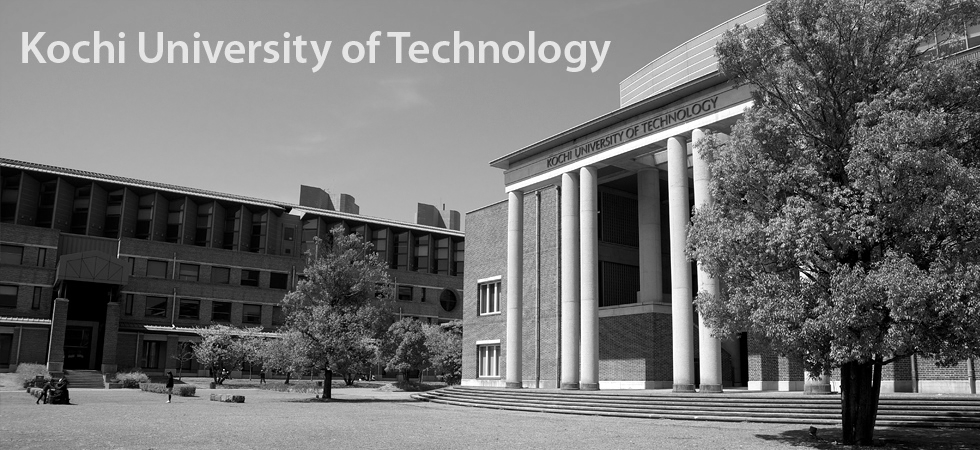
\includegraphics[keepaspectratio,width=\textwidth]{../../Figures/05_12_g.png}
        \subcaption{緑チャネル}
    \end{minipage}
    \begin{minipage}[b]{.19\textwidth}
        \centering
        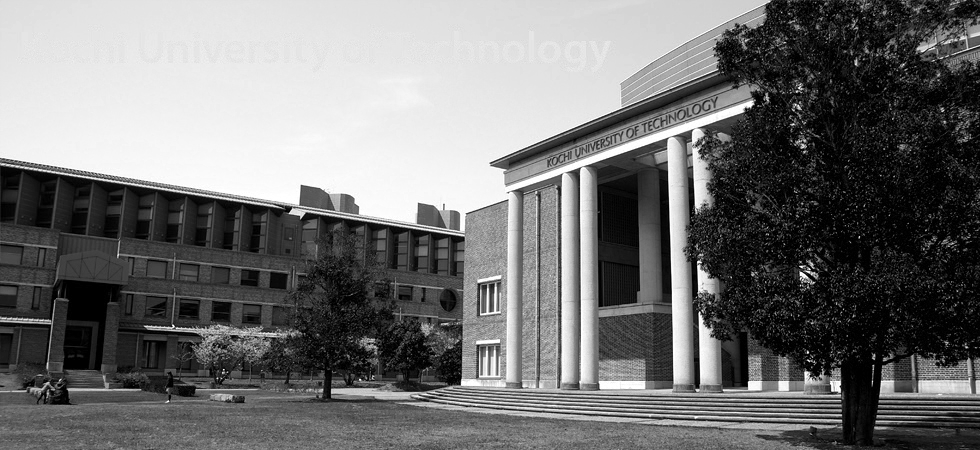
\includegraphics[keepaspectratio,width=\textwidth]{../../Figures/05_13_b.png}
        \subcaption{青チャネル}
    \end{minipage}
    \begin{minipage}[b]{.19\textwidth}
        \centering
        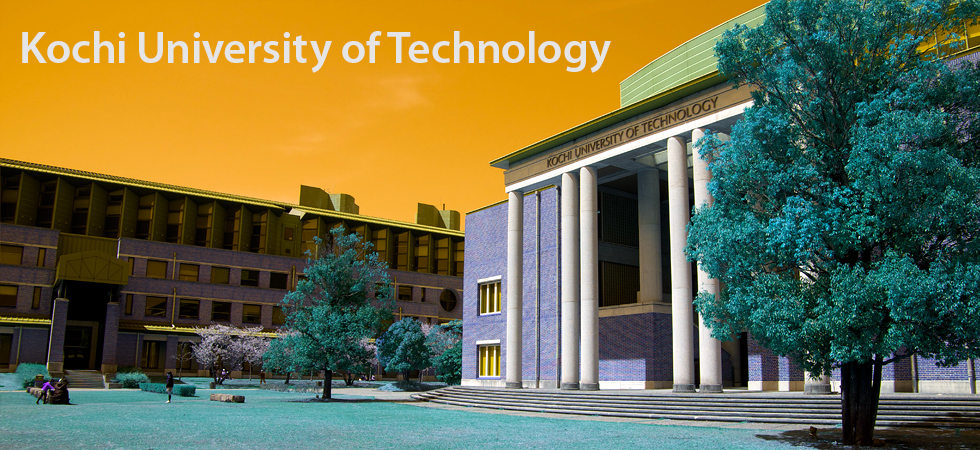
\includegraphics[keepaspectratio,width=\textwidth]{../../Figures/05_14_change.png}
        \subcaption{赤青チャネル入れ替え}
    \end{minipage}
    \caption{\kadaiaa\ 実験結果}
    \vsp
    \begin{minipage}[b]{.23\textwidth}
        \centering
        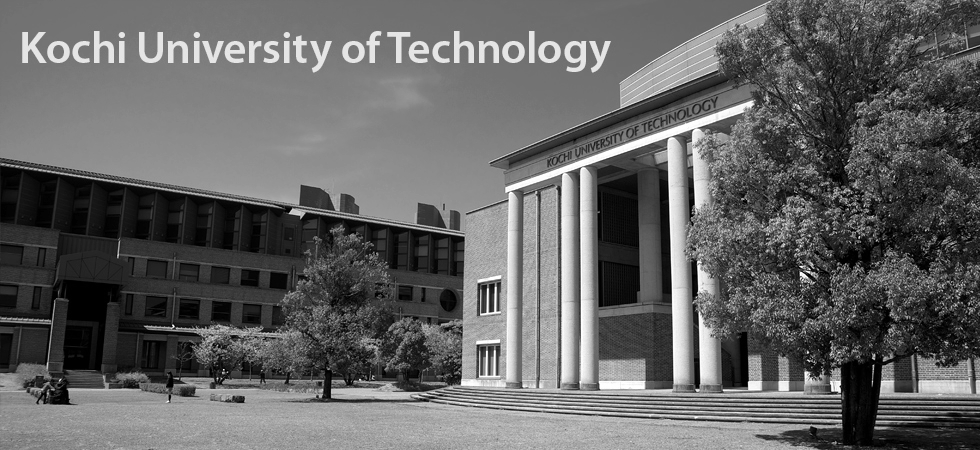
\includegraphics[keepaspectratio,width=\textwidth]{../../Figures/05_21_gimg.png}
        \subcaption{量子化数\ 8Bit\footnotemark[1]}
    \end{minipage}
    \begin{minipage}[b]{.23\textwidth}
        \centering
        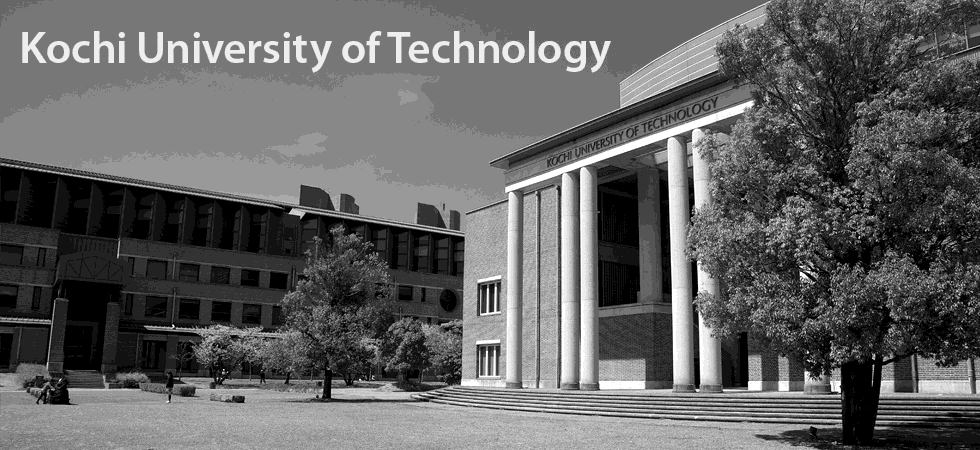
\includegraphics[keepaspectratio,width=\textwidth]{../../Figures/05_22_4bit.png}
        \subcaption{量子化数\ 4Bit}
    \end{minipage}
    \begin{minipage}[b]{.23\textwidth}
        \centering
        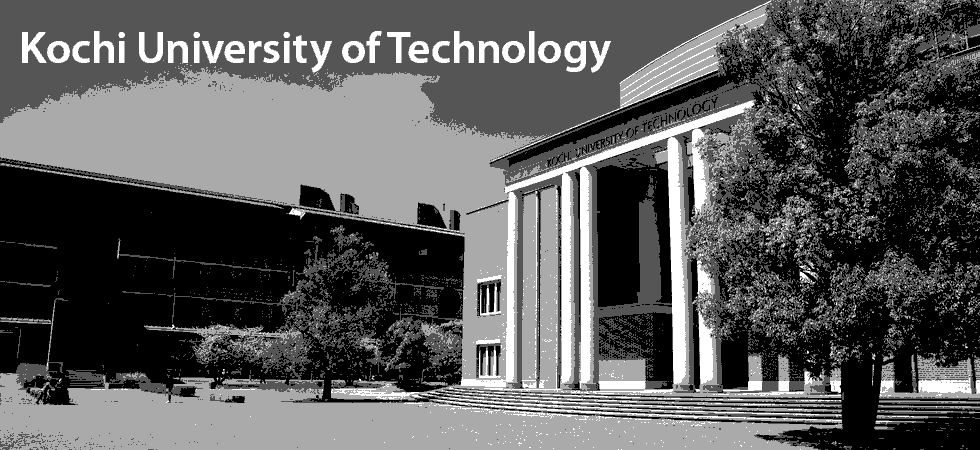
\includegraphics[keepaspectratio,width=\textwidth]{../../Figures/05_23_2bit.png}
        \subcaption{量子化数\ 2Bit}
    \end{minipage}
    \begin{minipage}[b]{.23\textwidth}
        \centering
        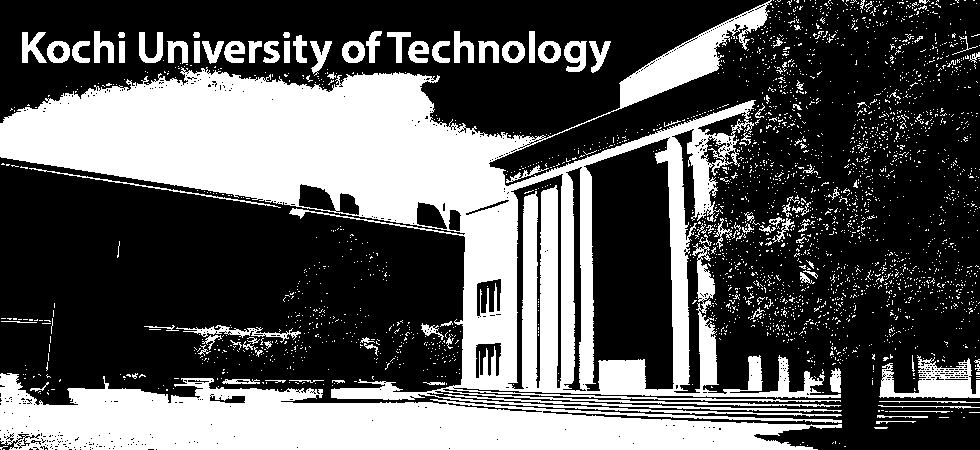
\includegraphics[keepaspectratio,width=\textwidth]{../../Figures/05_24_1bit.png}
        \subcaption{量子化数\ 1Bit}
    \end{minipage}
    \caption{\kadaiab\ 実験結果}
    \vsp
    \begin{minipage}[b]{.23\textwidth}
        \centering
        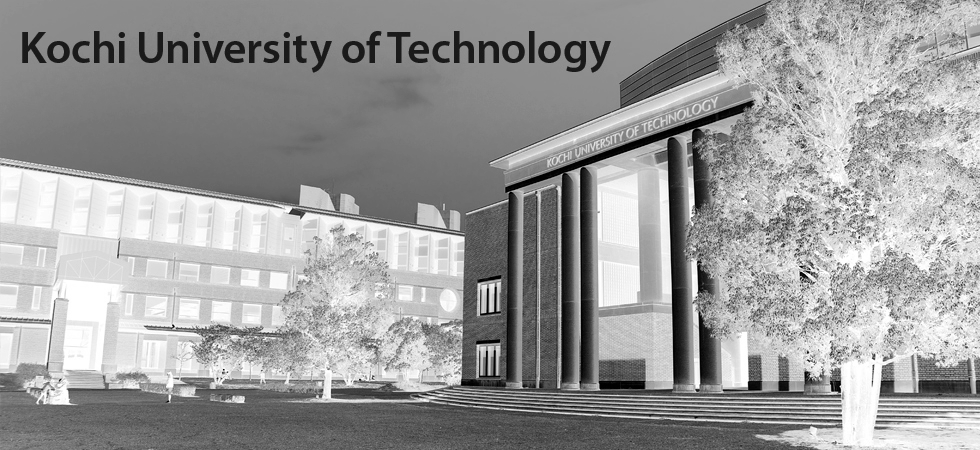
\includegraphics[keepaspectratio,width=\textwidth]{../../Figures/05_31_8.png}
        \subcaption{量子化数\ 8Bit}
    \end{minipage}
    \begin{minipage}[b]{.23\textwidth}
        \centering
        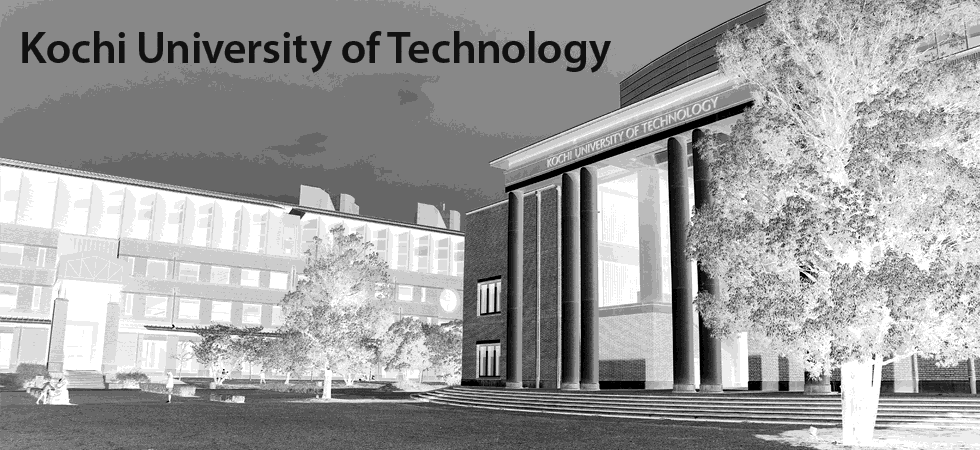
\includegraphics[keepaspectratio,width=\textwidth]{../../Figures/05_32_4.png}
        \subcaption{量子化数\ 4Bit}
    \end{minipage}
    \begin{minipage}[b]{.23\textwidth}
        \centering
        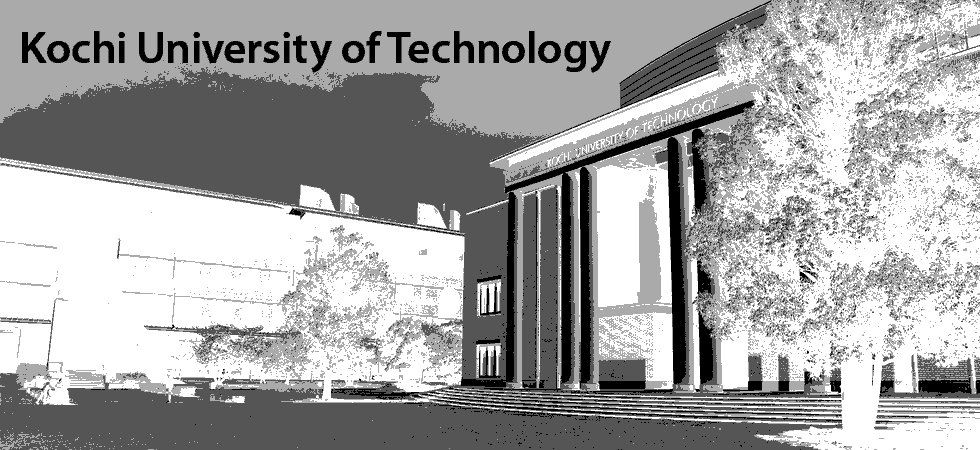
\includegraphics[keepaspectratio,width=\textwidth]{../../Figures/05_33_2.png}
        \subcaption{量子化数\ 2Bit}
    \end{minipage}
    \begin{minipage}[b]{.23\textwidth}
        \centering
        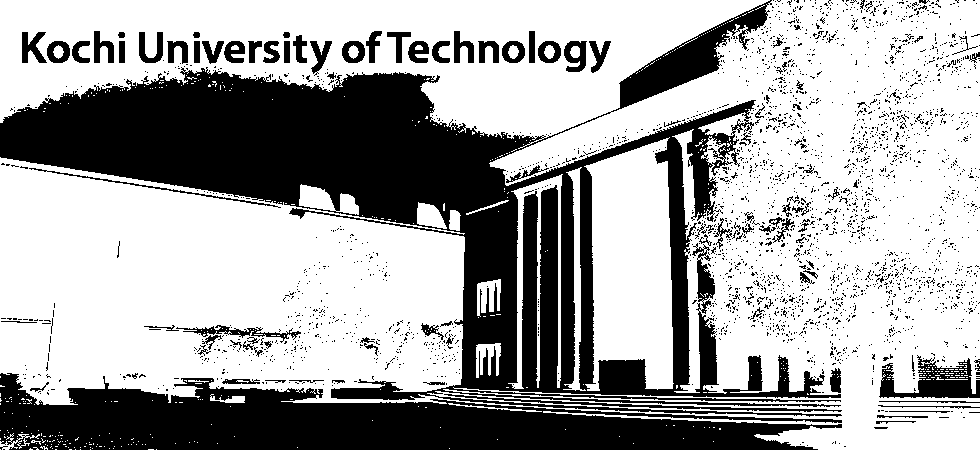
\includegraphics[keepaspectratio,width=\textwidth]{../../Figures/05_34_1.png}
        \subcaption{量子化数\ 1Bit}
    \end{minipage}
    \caption{\kadaiac\ 実験結果}
    \vsp
    \begin{minipage}[b]{.7\textwidth}
        \centering
        \begin{minipage}[b]{.3\textwidth}
            \centering
            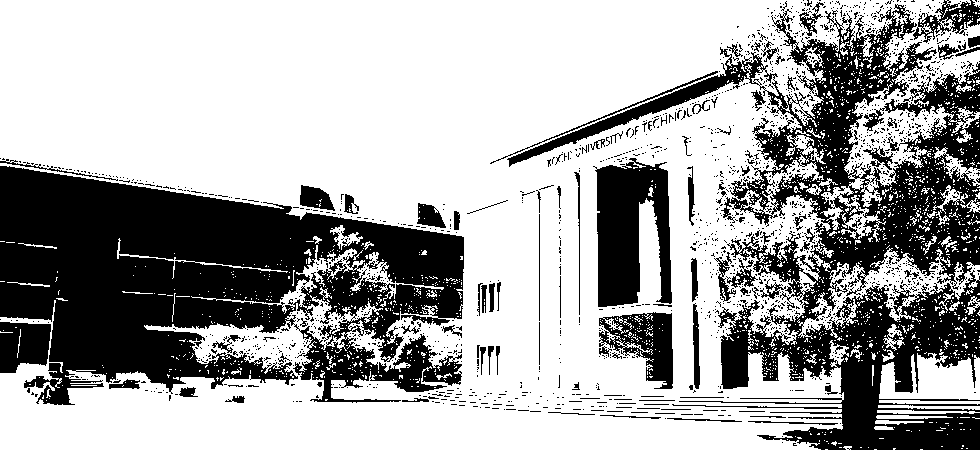
\includegraphics[keepaspectratio,width=\textwidth]{../../Figures/05_41.png}
            \subcaption{閾値\ \(64\)}
        \end{minipage}
        \begin{minipage}[b]{.3\textwidth}
            \centering
            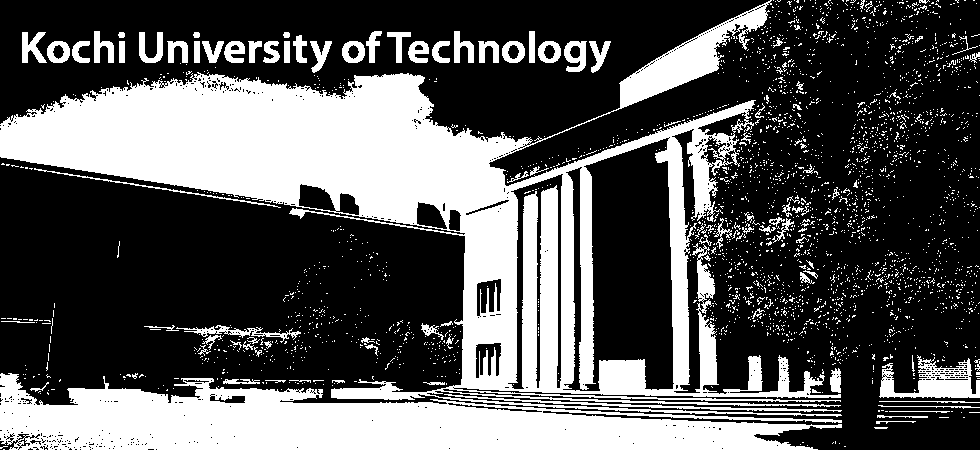
\includegraphics[keepaspectratio,width=\textwidth]{../../Figures/05_42.png}
            \subcaption{閾値\ \(128\)}
        \end{minipage}
        \begin{minipage}[b]{.3\textwidth}
            \centering
            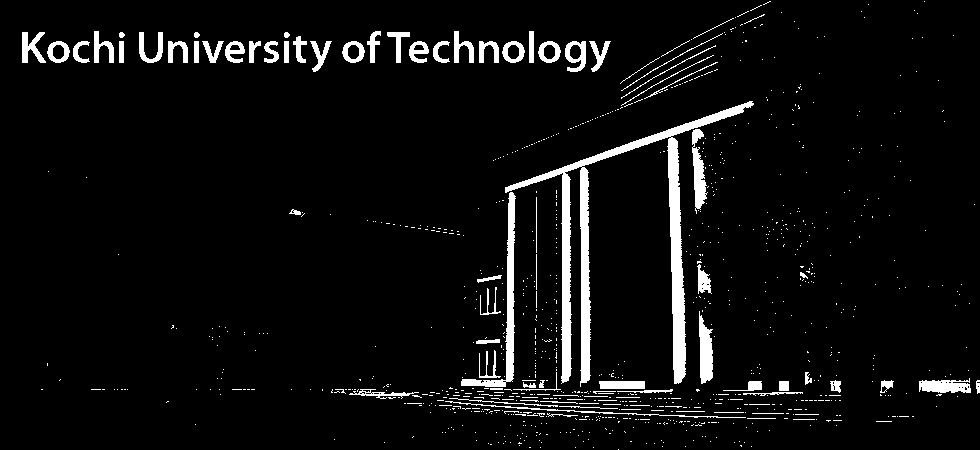
\includegraphics[keepaspectratio,width=\textwidth]{../../Figures/05_43.png}
            \subcaption{閾値\ \(192\)}
        \end{minipage}
        \caption{\kadaiad\ 実験結果}
    \end{minipage}
    \begin{minipage}[b]{.25\textwidth}
        \centering
        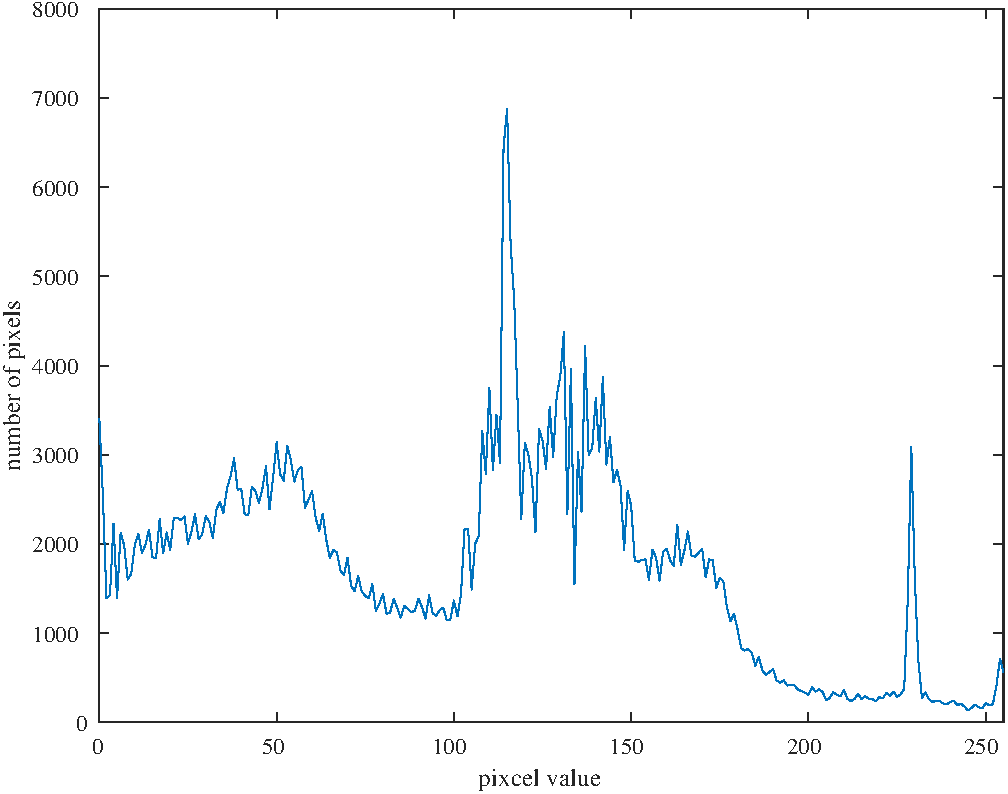
\includegraphics[keepaspectratio,width=\textwidth]{../../Figures/05_50_graph.pdf}
        \caption{\kadaiae\ 実験結果}
    \end{minipage}
    \nextfloat
    \\\vsp
    \begin{minipage}[b]{.49\textwidth}
        \centering
        \begin{minipage}[b]{.3\textwidth}
            \centering
            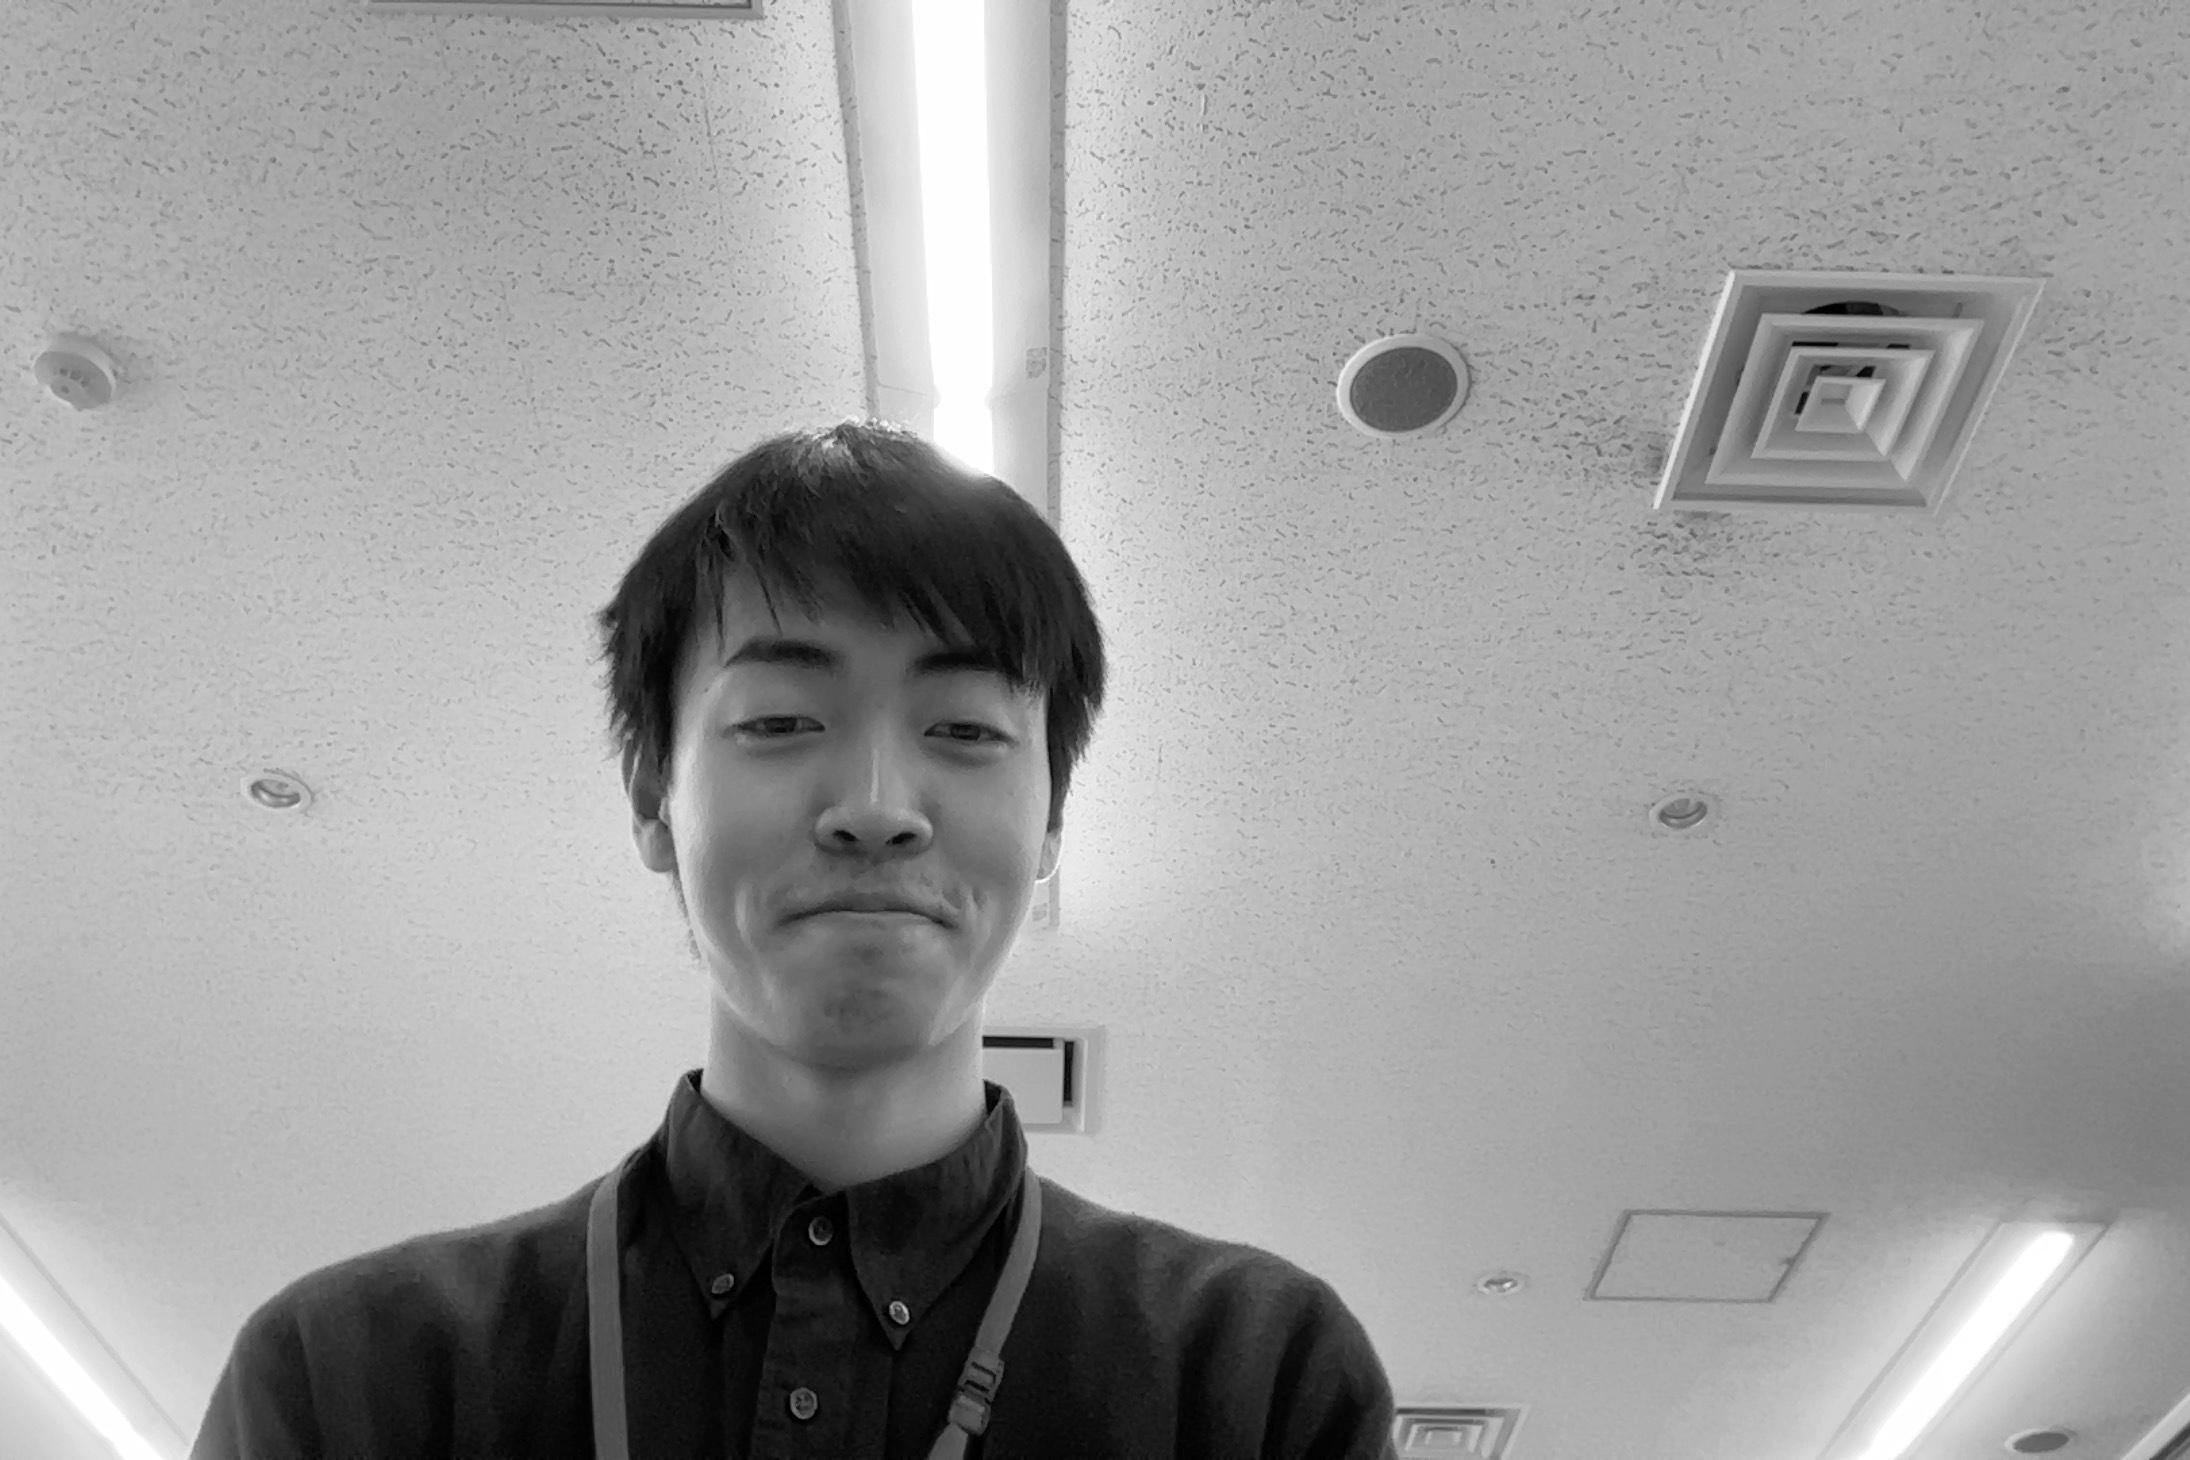
\includegraphics[keepaspectratio,width=\textwidth]{../../05_UnderstandingImages/fig1_g.jpg}
            \subcaption{被写体と背景}
        \end{minipage}
        \begin{minipage}[b]{.3\textwidth}
            \centering
            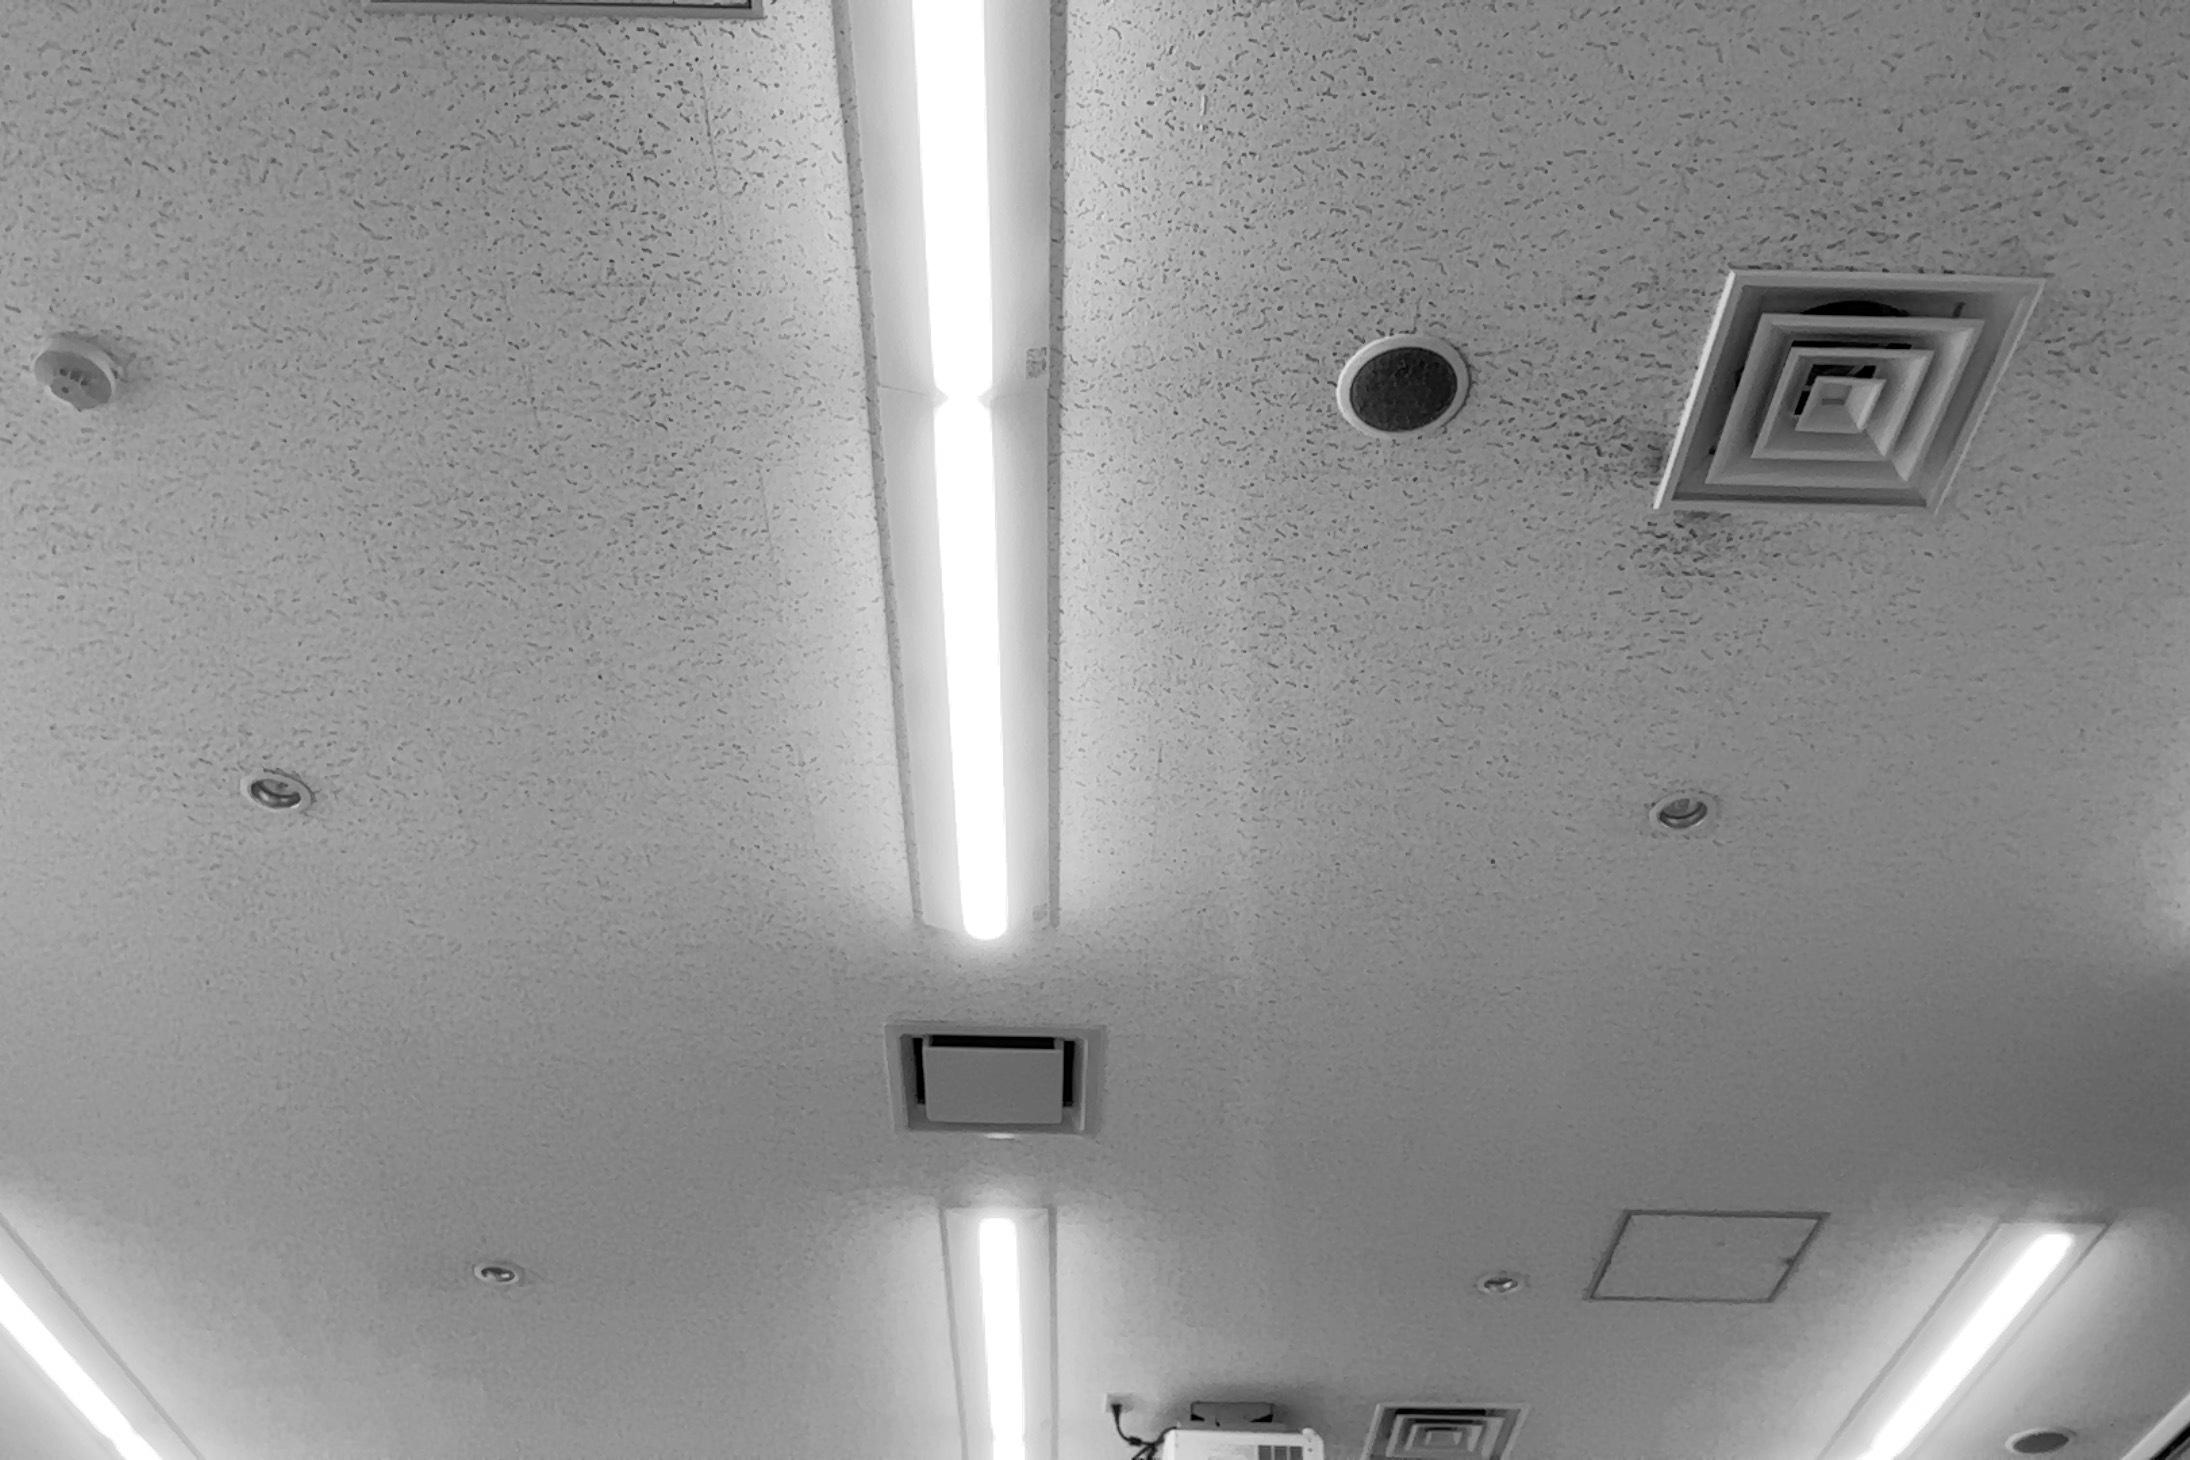
\includegraphics[keepaspectratio,width=\textwidth]{../../05_UnderstandingImages/fig2_g.jpg}
            \subcaption{背景のみ}
        \end{minipage}
        \begin{minipage}[b]{.3\textwidth}
            \centering
            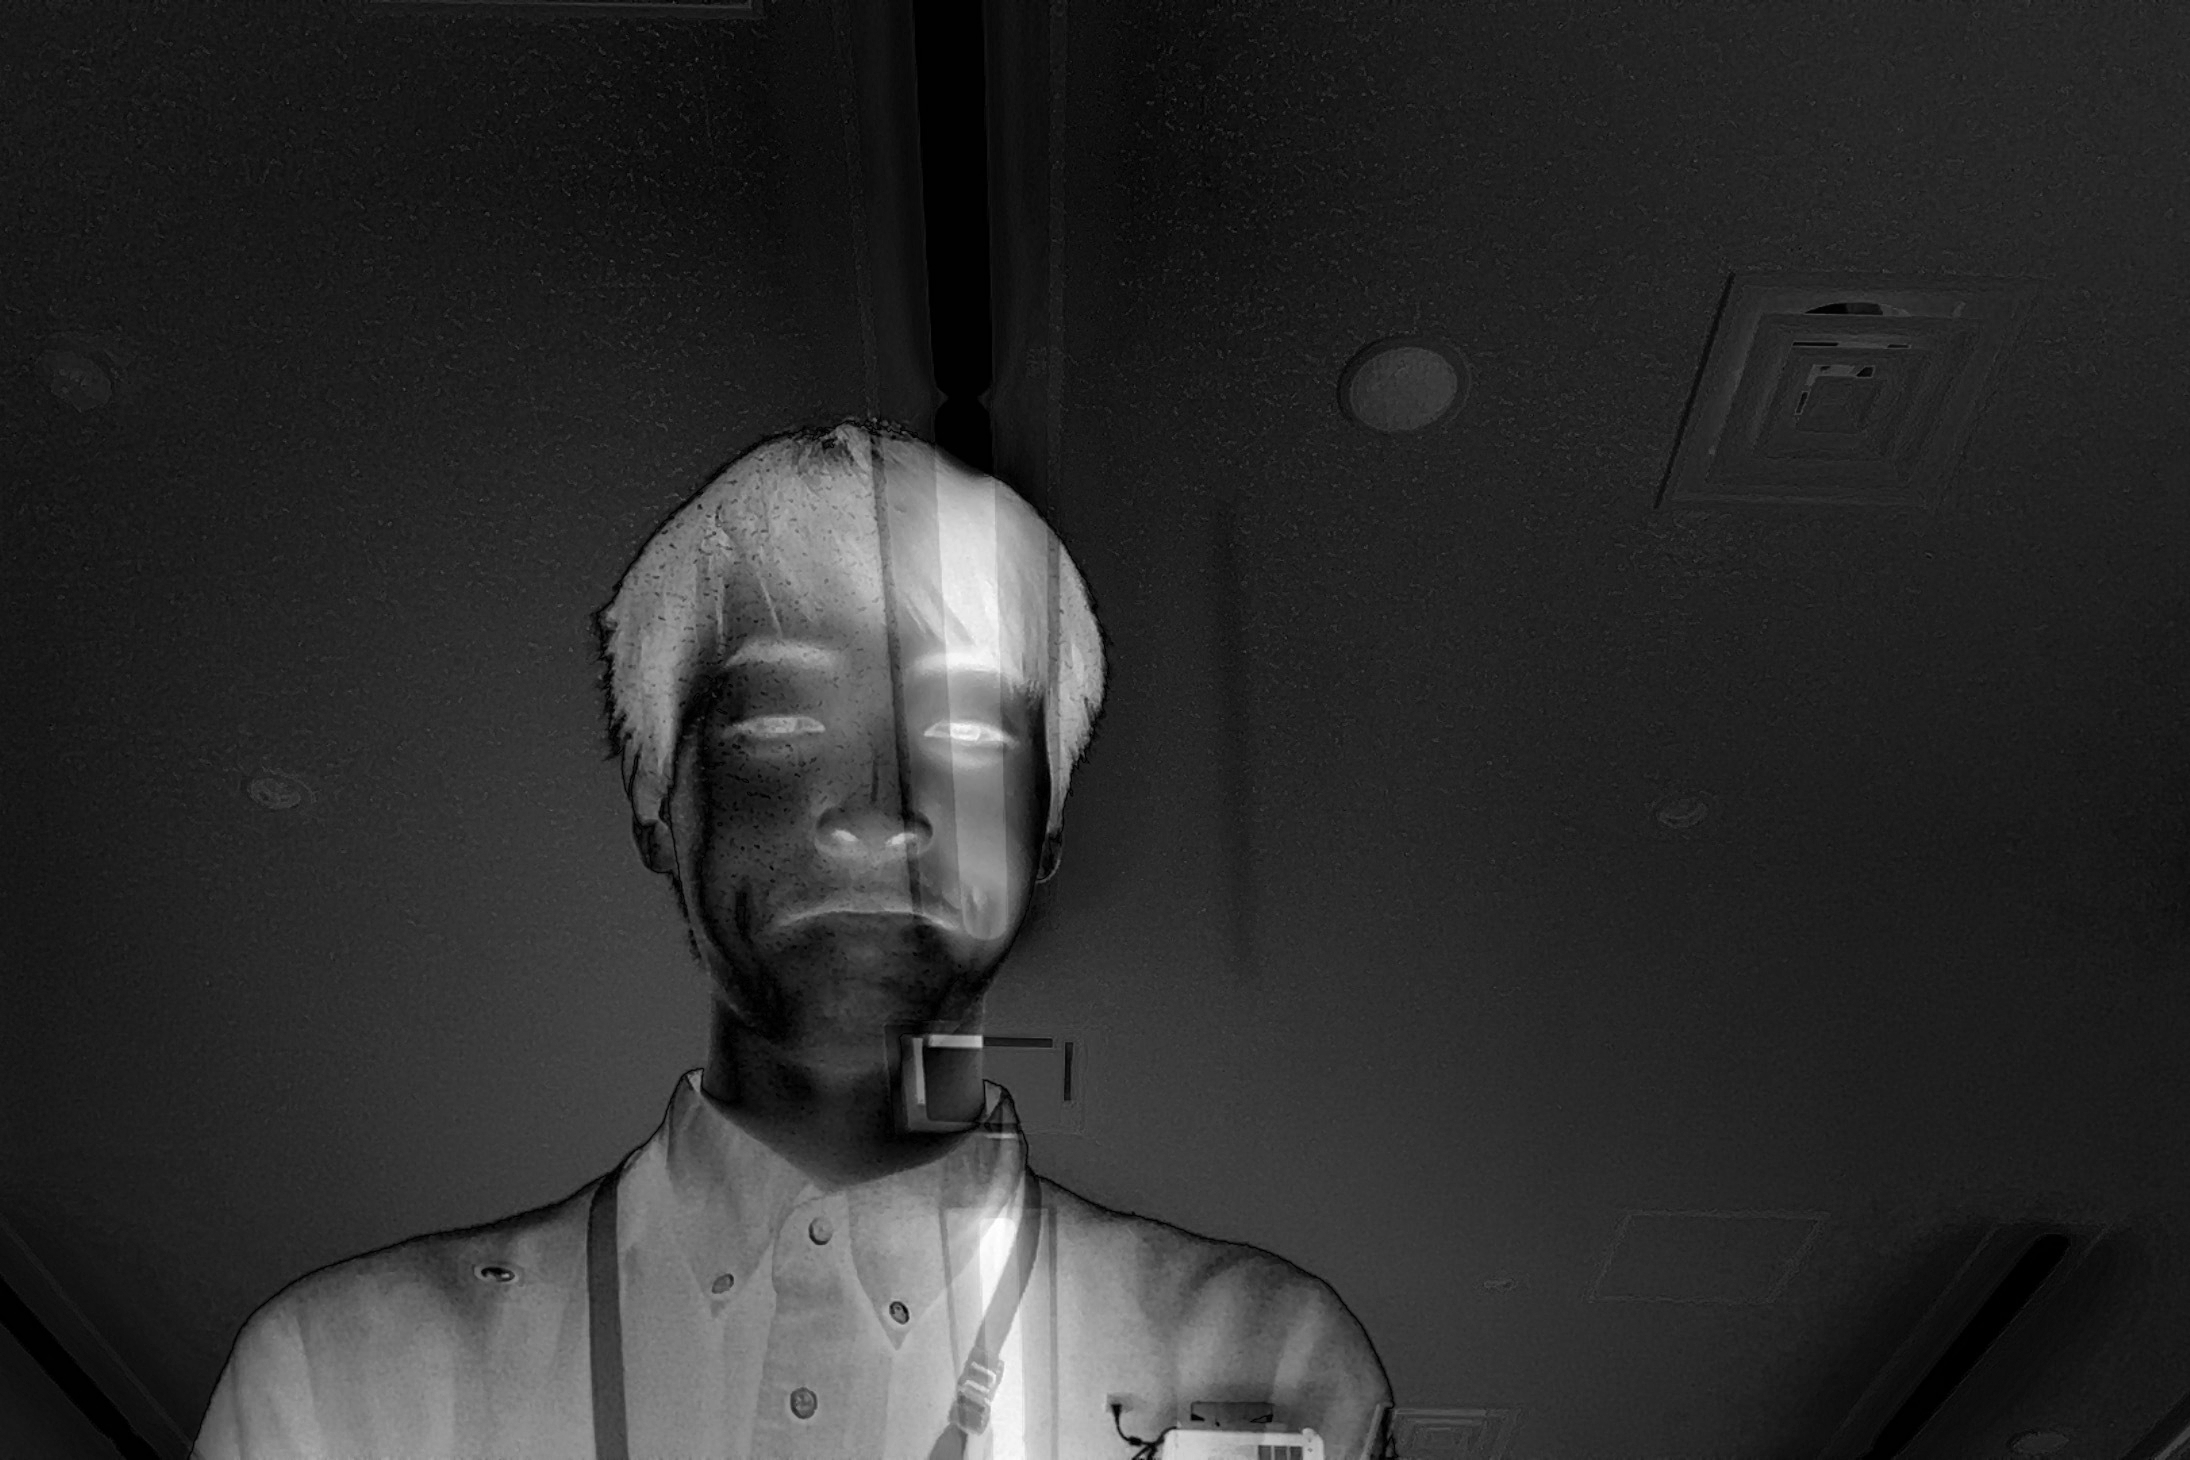
\includegraphics[keepaspectratio,width=\textwidth]{../../Figures/05_60.png}
            \subcaption{背景差分画像}
        \end{minipage}
        \caption{\kadaiaf\ 実験結果}
    \end{minipage}
    \nextfloat
    \begin{minipage}[b]{.49\textwidth}
        \centering
        \begin{minipage}[b]{.3\textwidth}
            \centering
            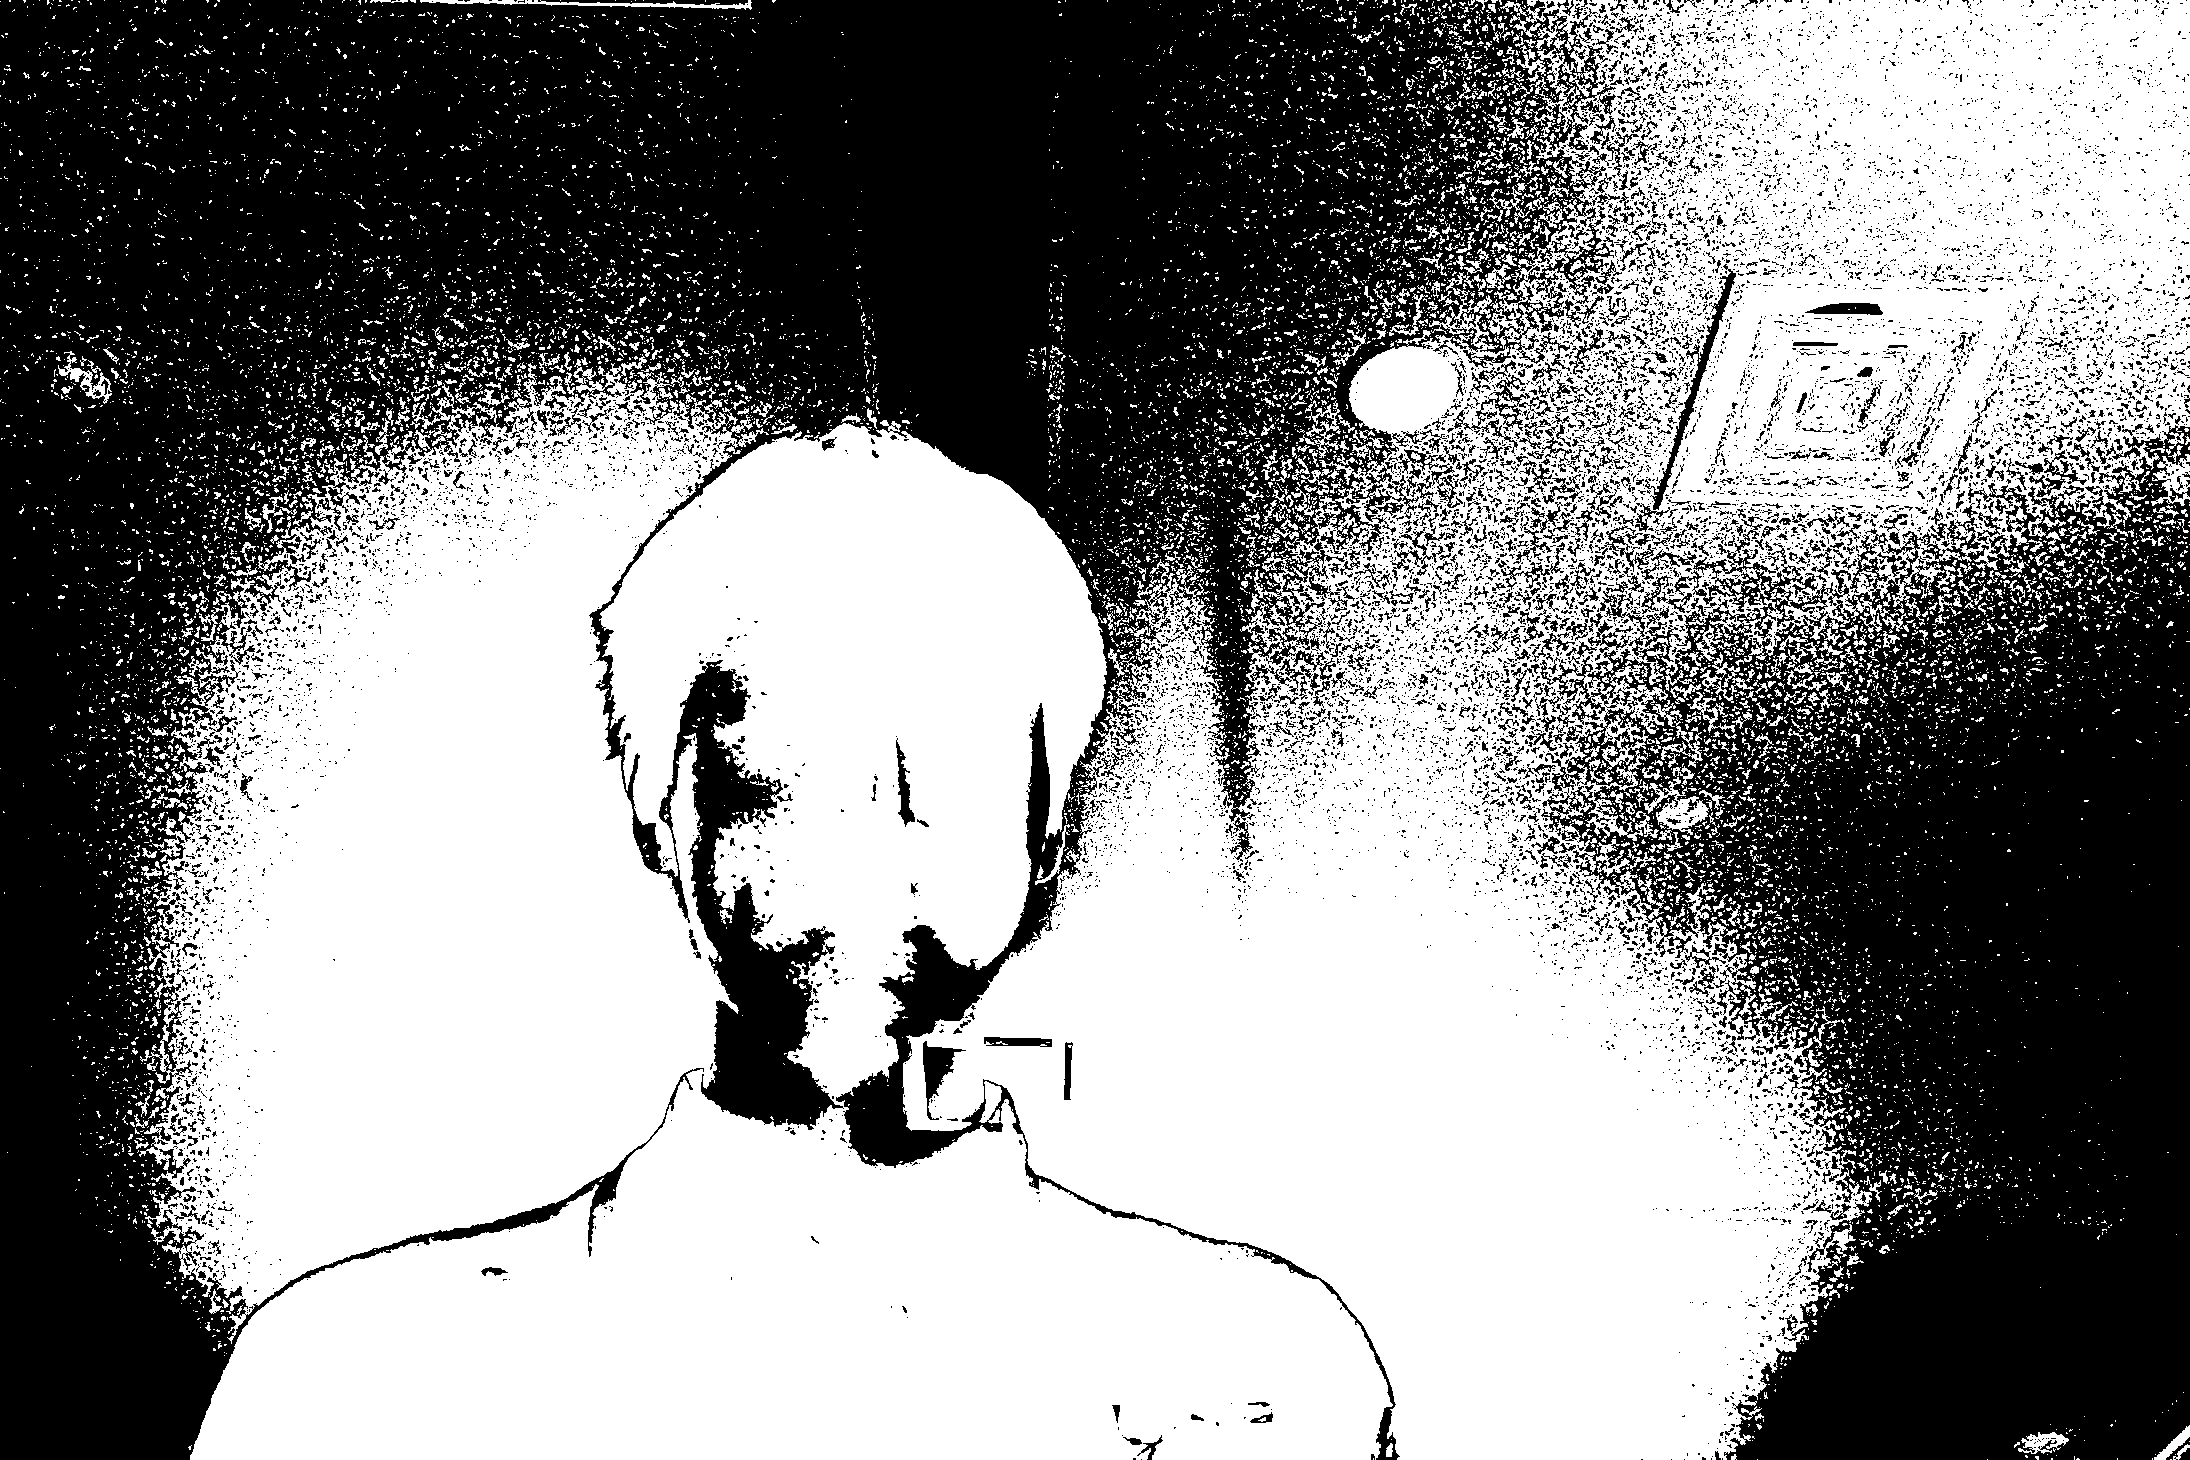
\includegraphics[keepaspectratio,width=\textwidth]{../../Figures/05_61.png}
            \subcaption{閾値\ \(32\)}
        \end{minipage}
        \begin{minipage}[b]{.3\textwidth}
            \centering
            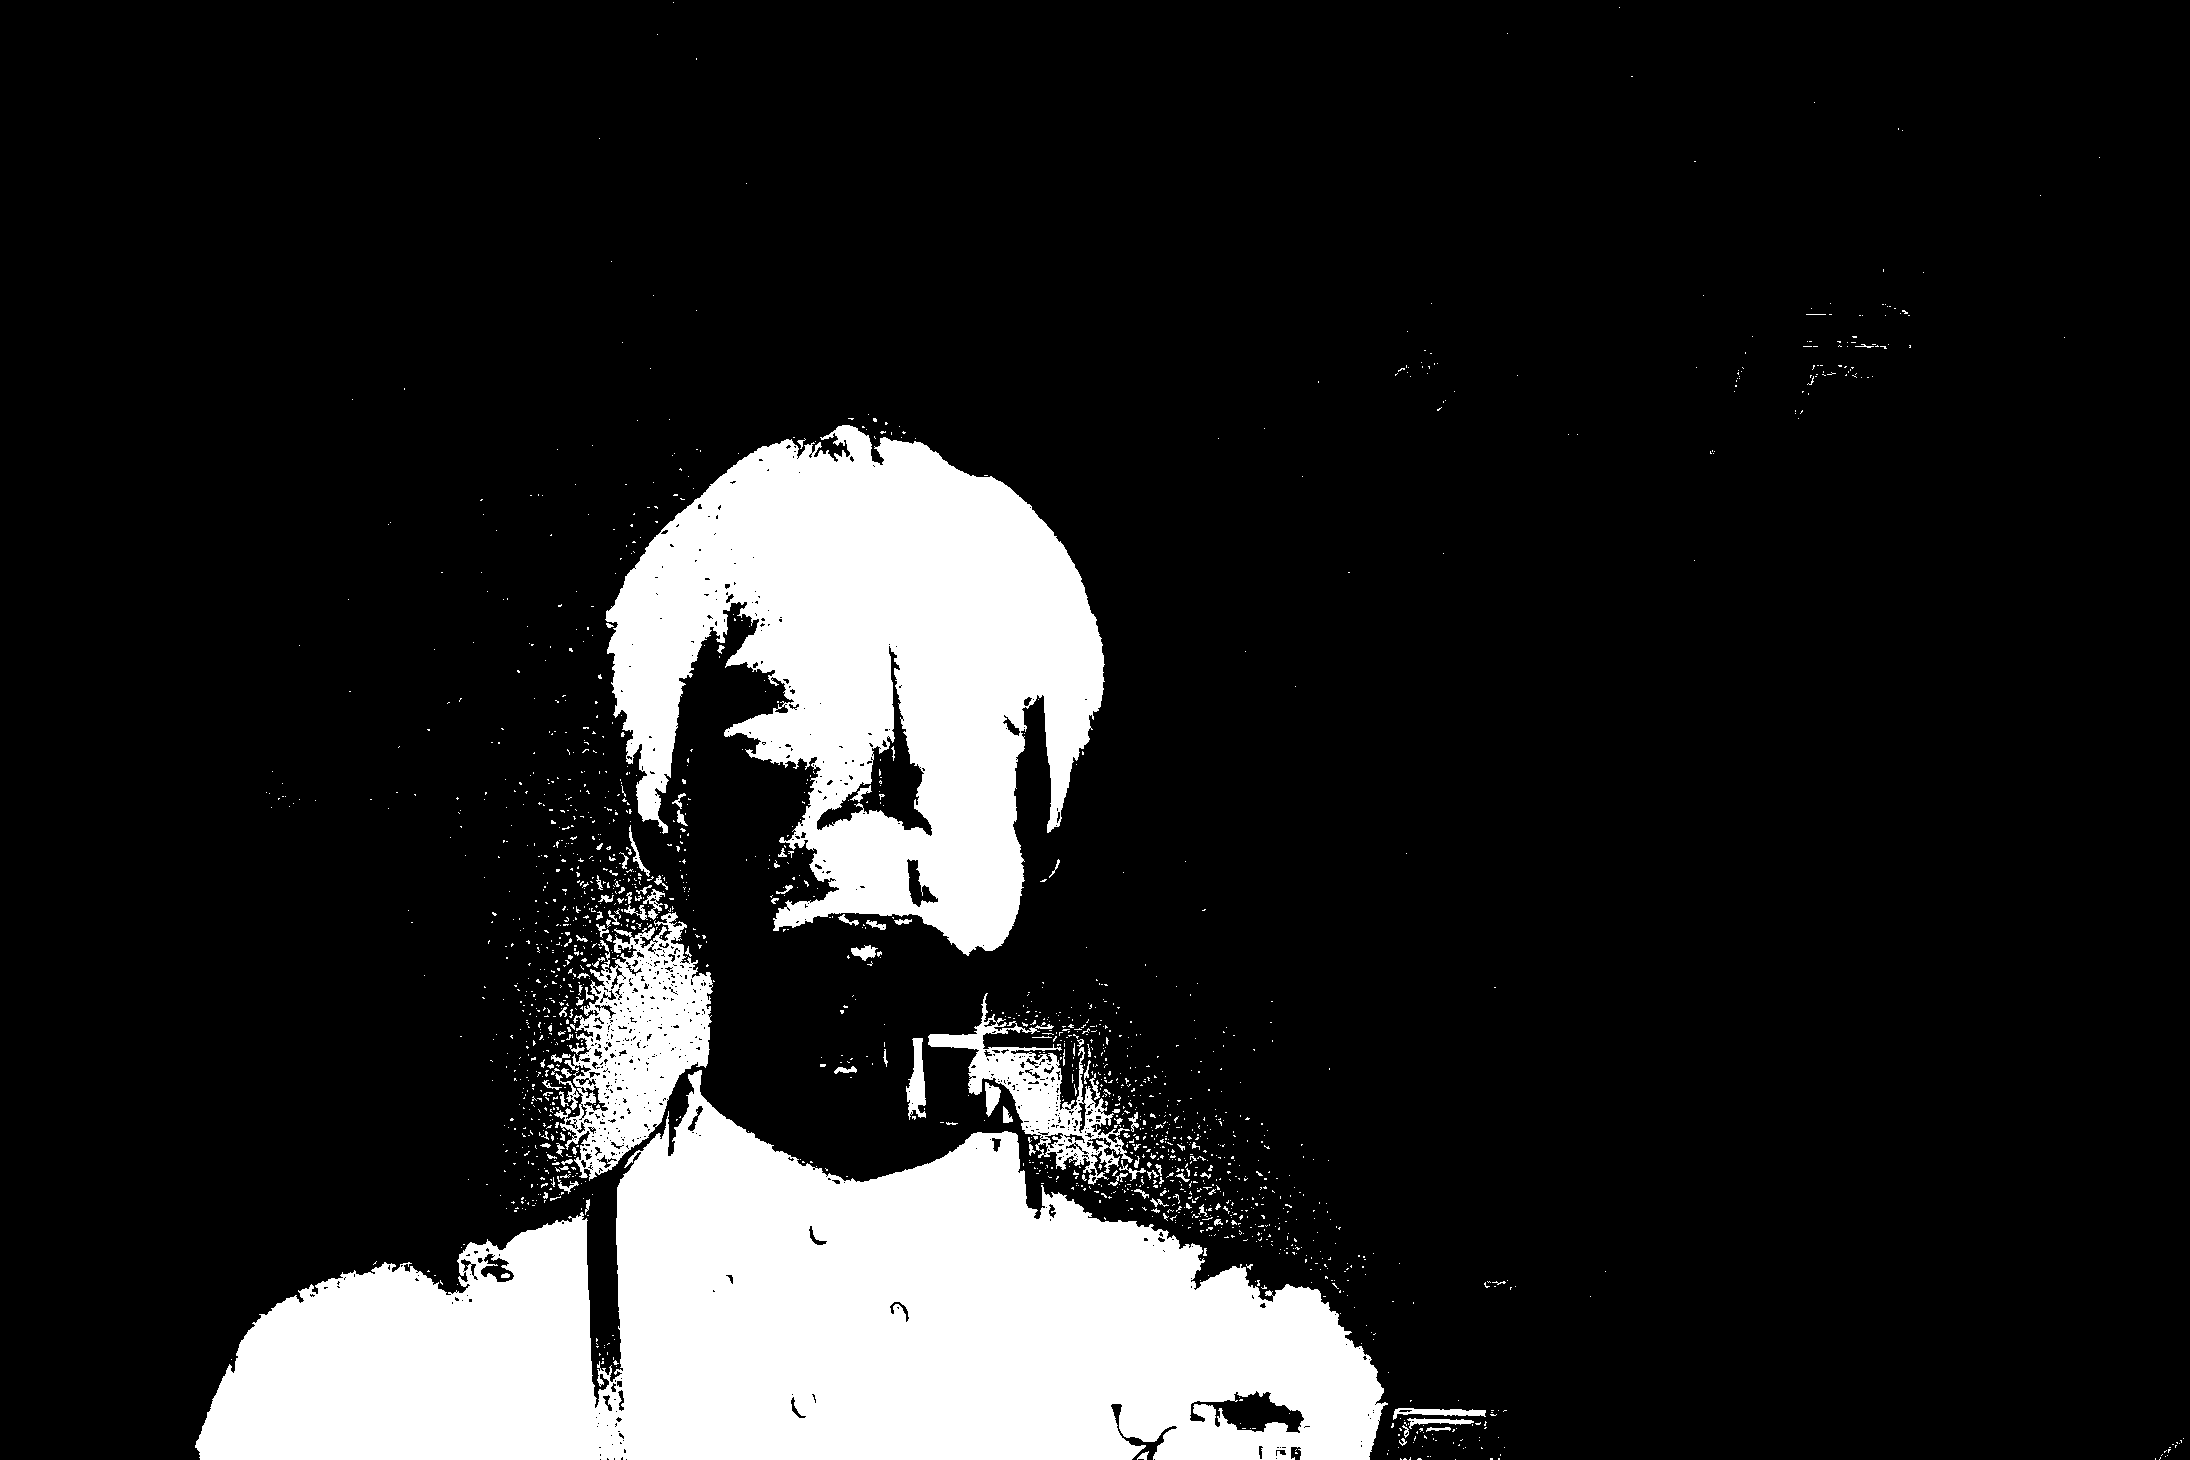
\includegraphics[keepaspectratio,width=\textwidth]{../../Figures/05_62.png}
            \subcaption{閾値\ \(64\)}
        \end{minipage}
        \begin{minipage}[b]{.3\textwidth}
            \centering
            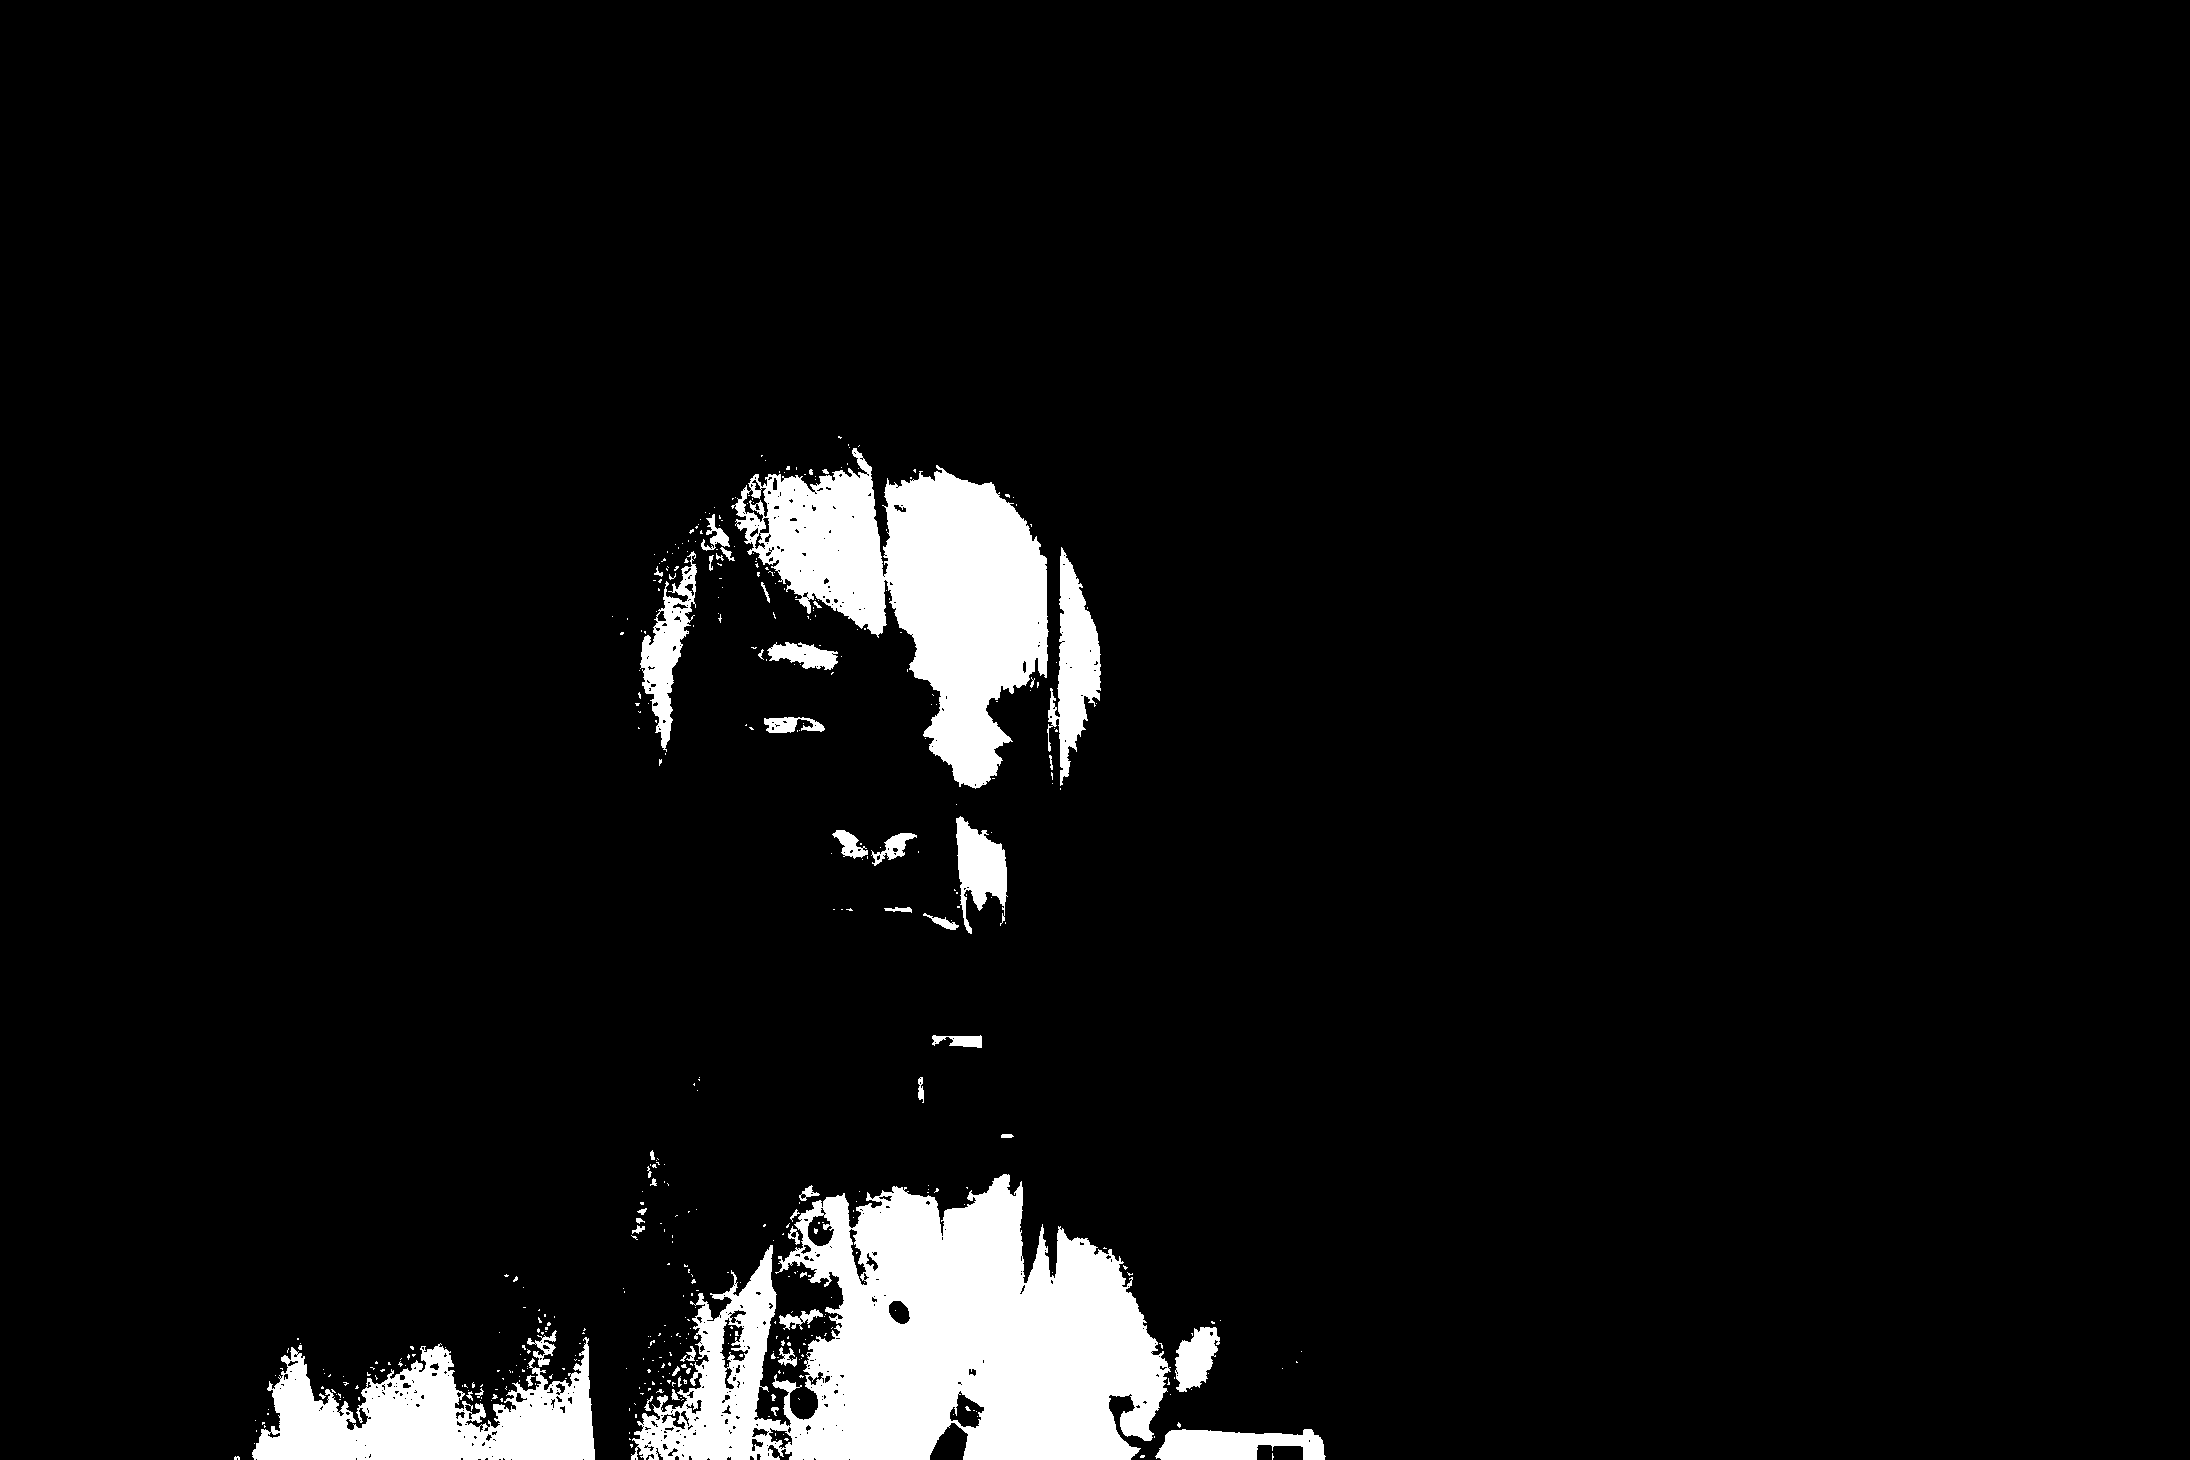
\includegraphics[keepaspectratio,width=\textwidth]{../../Figures/05_63.png}
            \subcaption{閾値\ \(128\)}
        \end{minipage}
        \caption{背景差分画像の閾値処理}
    \end{minipage}
\end{figure}
\footnotetext[1]{NTSC輝度信号のグレイスケール画像}
\section{\consideration}
\paragraph{\kadaiaa}
実験結果より,原画像に近い画像は,緑チャネルだけを抜き出してグレイスケール画像として表示したものである.
また,赤チャネルと青チャネルを入れ替えた画像では,文字や建物の概形を,はっきりとらえることができる.
これらは,\eqref{equ:grayscale}でGreenの割合が一番多い理由と考えられる.
\paragraph{\kadaiab}
量子化数を減らすことで,等高線のようなものが見える.
これは,元画像でなだらかな画素値の変化箇所が,量子化数を減らすことでとびとびの値になることで生じる.これを擬似輪郭という.
擬似輪郭は,量子化数を減らすことでより顕著になる.
\paragraph{\kadaiac}
量子化数が減ると擬似輪郭が生じる.この擬似輪郭は,階調反転しても変わらない.
\paragraph{\kadaiad}
閾値を調節することで,擬似輪郭を境に白と黒に別れることがわかった.
\paragraph{\kadaiaf}
背景差分画像では,被写体がぼんやりと写っている.この画像に対して閾値処理することで,被写体を強調できることが分かった.
